% This LaTeX was auto-generated from MATLAB code.
% To make changes, update the MATLAB code and export to LaTeX again.

\documentclass{article}

\usepackage[utf8]{inputenc}
\usepackage[T1]{fontenc}
\usepackage{lmodern}
\usepackage{graphicx}
\usepackage{color}
\usepackage{hyperref}
\usepackage{amsmath}
\usepackage{amsfonts}
\usepackage{epstopdf}
\usepackage[table]{xcolor}
\usepackage{matlab}

\sloppy
\epstopdfsetup{outdir=./}
\graphicspath{ {./HW12_code_images/} }

\matlabhastoc

\matlabmultipletitles

\begin{document}

\maketitle
\thispagestyle{empty}
\pagebreak
\matlabtableofcontents{Table of Contents}

\begin{par}
\begin{flushleft}
In the first problem of this homework assignment a Radial Basis Function neural network will be trained on MNIST dataset and its classification performance will be reported.
\end{flushleft}
\end{par}

\begin{par}
\begin{flushleft}
The second problem discussed how to find the partial derivatives to be used on gradient descent algorithm.
\end{flushleft}
\end{par}

\begin{matlabcode}
clc; clear; close all;
load('HW12_code_workspace.mat');
\end{matlabcode}
\pagebreak

\label{T_AF22880B}
\matlabtitle{MNIST Dataset}

\label{H_FBA02D0E}
\matlabheading{0.1 Downloading MNIST Dataset and Import into \textit{Matlab}}

\begin{par}
\begin{flushleft}
The code snippet below will download MNIST dataset from web and extract the downloaded files into Matlab matrices as test and train images and labels.
\end{flushleft}
\end{par}

\begin{matlabcode}
mnist_train_image = 'train-images-idx3-ubyte';
mnist_train_label = 'train-labels-idx1-ubyte';
mnist_test_image  = 't10k-images-idx3-ubyte';
mnist_test_label  = 't10k-labels-idx1-ubyte';
train_set_number  = 60000;
test_set_number   = 10000;

downloadMNIST(mnist_train_image, mnist_train_label, mnist_test_image, mnist_test_label);
\end{matlabcode}
\begin{matlaboutput}
Downloading MNIST dataset...
MNIST dataset downloded.
Unzipping started...
Unzipping completed.
\end{matlaboutput}


\begin{matlabcode}
[train_images, train_labels] = readMNIST(mnist_train_image, mnist_train_label, train_set_number);
[test_images,   test_labels] = readMNIST(mnist_test_image, mnist_test_label, test_set_number);

clear mnist_train_image mnist_train_label mnist_test_image mnist_test_label train_set_number test_set_number
\end{matlabcode}


\label{H_3C76610B}
\matlabheading{0.2 Plotting a Sample of MNIST Dataset}

\begin{par}
\begin{flushleft}
A set of 100 randomly chosen samples of the training dataset is plotted here.
\end{flushleft}
\end{par}

\begin{matlabcode}
random_indices = randi(60000, [1 100]);
montage(train_images(:, :, random_indices), 'BorderSize', [2 2], 'BackgroundColor', 'white');
\end{matlabcode}
\begin{center}
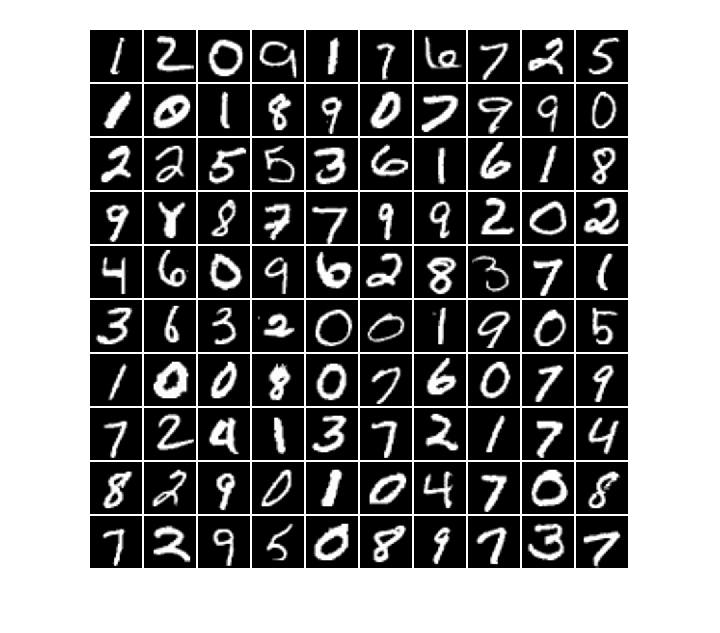
\includegraphics[scale=0.6]{figure_0.png}
\end{center}


\label{H_FC5FEF34}
\matlabheading{0.3 Number of Occurances for Each Digit in Training Set}

\begin{par}
\begin{flushleft}
Here we investigate how many of each digit is there in the training set.
\end{flushleft}
\end{par}

\begin{matlabcode}
for i=0:9
    disp([num2str(i),': ', num2str(sum(train_labels == i))]);
end
\end{matlabcode}
\begin{matlaboutput}
0: 5923
1: 6742
2: 5958
3: 6131
4: 5842
5: 5421
6: 5918
7: 6265
8: 5851
9: 5949
\end{matlaboutput}


\label{H_E5B0FAB6}
\matlabheading{0.4 Rashaping Images Into Vectors}

\begin{par}
\begin{flushleft}
For further calculations it is more desirable to work with vectors of 784 elements instead of 28x28 size images.
\end{flushleft}
\end{par}

\begin{matlabcode}
train_images_reshaped = reshape(train_images, [size(train_images, 1)*size(train_images, 2) size(train_images, 3)]);
test_images_reshaped = reshape(test_images, [size(test_images, 1)*size(test_images, 2) size(test_images, 3)]);
\end{matlabcode}
\pagebreak

\label{T_F3C18C75}
\matlabtitle{Problem 1}

\begin{par}
\begin{flushleft}
In this problem we implement an RBF network with 40 hidden units and 10 binary outputs.
\end{flushleft}
\end{par}

\label{H_2FA366D7}
\matlabheading{1.1 Finding Centroids Using K-means Clustring Algorithm}

\begin{par}
\begin{flushleft}
By running a K-means algorithm on the training dataset, we have found 40 centroids to be used later in the radial basis functions.
\end{flushleft}
\end{par}

\begin{matlabcode}
K = 40;
[idx, centroids] = kmeans(train_images_reshaped', K, "Display", "iter", "MaxIter", 1000, 'OnlinePhase','on');
\end{matlabcode}
\begin{matlaboutput}
  iter	 phase	     num	         sum
     1	     1	   60000	 2.17743e+06
     2	     1	   17400	 2.03712e+06
     3	     1	    8921	 1.99709e+06
     4	     1	    5806	 1.97847e+06
     5	     1	    4445	 1.96579e+06
     6	     1	    3544	 1.95701e+06
     7	     1	    2930	 1.95091e+06
     8	     1	    2449	 1.94653e+06
     9	     1	    2030	 1.94354e+06
    10	     1	    1667	  1.9415e+06
    11	     1	    1454	 1.93993e+06
    12	     1	    1216	 1.93875e+06
    13	     1	    1124	 1.93772e+06
    14	     1	    1058	  1.9368e+06
    15	     1	     960	 1.93605e+06
    16	     1	     933	 1.93534e+06
    17	     1	     853	 1.93469e+06
    18	     1	     884	 1.93397e+06
    19	     1	     893	 1.93322e+06
    20	     1	     919	 1.93239e+06
    21	     1	     947	 1.93141e+06
    22	     1	     949	 1.93028e+06
    23	     1	    1020	  1.9288e+06
    24	     1	    1066	   1.927e+06
    25	     1	     998	 1.92553e+06
    26	     1	     908	 1.92448e+06
    27	     1	     863	 1.92363e+06
    28	     1	     775	 1.92301e+06
    29	     1	     714	 1.92253e+06
    30	     1	     619	 1.92211e+06
    31	     1	     576	 1.92178e+06
    32	     1	     526	  1.9215e+06
    33	     1	     529	 1.92122e+06
    34	     1	     530	 1.92094e+06
    35	     1	     497	 1.92068e+06
    36	     1	     510	 1.92042e+06
    37	     1	     512	 1.92016e+06
    38	     1	     462	 1.91993e+06
    39	     1	     447	 1.91972e+06
    40	     1	     460	 1.91951e+06
    41	     1	     447	 1.91928e+06
    42	     1	     462	 1.91906e+06
    43	     1	     414	 1.91887e+06
    44	     1	     421	 1.91865e+06
    45	     1	     410	 1.91843e+06
    46	     1	     380	 1.91824e+06
    47	     1	     377	 1.91804e+06
    48	     1	     366	 1.91786e+06
    49	     1	     400	 1.91762e+06
    50	     1	     411	 1.91738e+06
    51	     1	     407	 1.91712e+06
    52	     1	     459	 1.91682e+06
    53	     1	     486	 1.91647e+06
    54	     1	     503	 1.91609e+06
    55	     1	     507	 1.91573e+06
    56	     1	     508	 1.91536e+06
    57	     1	     530	 1.91497e+06
    58	     1	     533	 1.91458e+06
    59	     1	     496	 1.91424e+06
    60	     1	     490	 1.91391e+06
    61	     1	     468	 1.91358e+06
    62	     1	     475	 1.91328e+06
    63	     1	     472	 1.91298e+06
    64	     1	     470	 1.91269e+06
    65	     1	     433	 1.91247e+06
    66	     1	     397	 1.91227e+06
    67	     1	     373	  1.9121e+06
    68	     1	     342	 1.91197e+06
    69	     1	     271	 1.91188e+06
    70	     1	     240	 1.91182e+06
    71	     1	     245	 1.91175e+06
    72	     1	     207	  1.9117e+06
    73	     1	     198	 1.91165e+06
    74	     1	     192	 1.91159e+06
    75	     1	     206	 1.91154e+06
    76	     1	     209	 1.91148e+06
    77	     1	     214	  1.9114e+06
    78	     1	     202	 1.91134e+06
    79	     1	     208	 1.91127e+06
    80	     1	     191	 1.91119e+06
    81	     1	     184	 1.91113e+06
    82	     1	     189	 1.91107e+06
    83	     1	     191	   1.911e+06
    84	     1	     190	 1.91094e+06
    85	     1	     177	 1.91089e+06
    86	     1	     176	 1.91083e+06
    87	     1	     166	 1.91077e+06
    88	     1	     158	 1.91072e+06
    89	     1	     162	 1.91067e+06
    90	     1	     174	 1.91062e+06
    91	     1	     172	 1.91057e+06
    92	     1	     166	 1.91052e+06
    93	     1	     148	 1.91047e+06
    94	     1	     145	 1.91043e+06
    95	     1	     105	 1.91041e+06
    96	     1	     116	 1.91038e+06
    97	     1	     101	 1.91036e+06
    98	     1	     123	 1.91033e+06
    99	     1	     132	  1.9103e+06
   100	     1	     126	 1.91027e+06
   101	     1	     104	 1.91025e+06
   102	     1	      86	 1.91023e+06
   103	     1	      79	 1.91022e+06
   104	     1	      69	 1.91021e+06
   105	     1	      58	  1.9102e+06
   106	     1	      50	 1.91019e+06
   107	     1	      50	 1.91018e+06
   108	     1	      41	 1.91018e+06
   109	     1	      24	 1.91018e+06
   110	     1	      24	 1.91017e+06
   111	     1	      28	 1.91017e+06
   112	     1	      29	 1.91017e+06
   113	     1	      31	 1.91017e+06
   114	     1	      25	 1.91016e+06
   115	     1	      16	 1.91016e+06
   116	     1	      18	 1.91016e+06
   117	     1	      16	 1.91016e+06
   118	     1	      15	 1.91016e+06
   119	     1	      11	 1.91015e+06
   120	     1	       8	 1.91015e+06
   121	     1	       2	 1.91015e+06
   122	     1	       1	 1.91015e+06
   123	     2	       1	 1.91015e+06
   124	     2	       1	 1.91014e+06
   125	     2	       1	 1.91014e+06
   126	     2	       1	 1.91013e+06
   127	     2	       1	 1.91013e+06
   128	     2	       1	 1.91012e+06
   129	     2	       1	 1.91011e+06
   130	     2	       1	 1.91011e+06
   131	     2	       1	  1.9101e+06
   132	     2	       1	  1.9101e+06
   133	     2	       1	 1.91009e+06
   134	     2	       1	 1.91009e+06
   135	     2	       1	 1.91008e+06
   136	     2	       1	 1.91008e+06
   137	     2	       1	 1.91008e+06
   138	     2	       1	 1.91008e+06
   139	     2	       1	 1.91008e+06
   140	     2	       1	 1.91008e+06
   141	     2	       0	 1.91008e+06
Best total sum of distances = 1.91008e+06
\end{matlaboutput}
\pagebreak

\begin{par}
\begin{flushleft}
The 40 centroids are plotted below:
\end{flushleft}
\end{par}

\begin{matlabcode}
iMontage(centroids');
\end{matlabcode}
\begin{center}
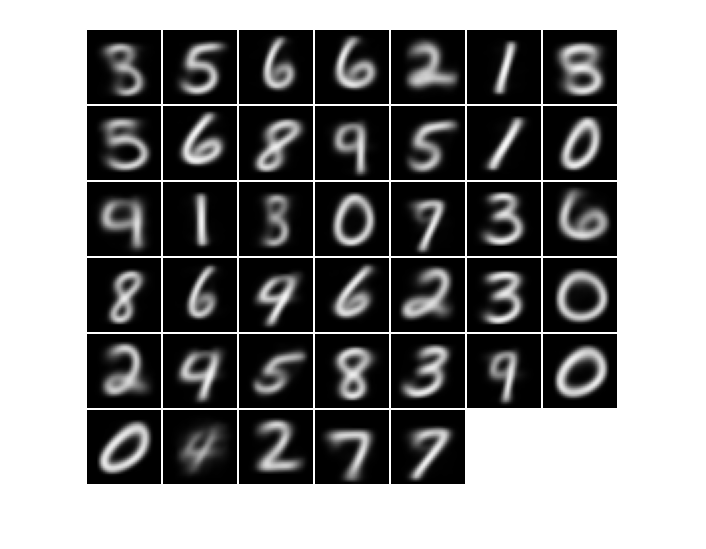
\includegraphics[width=\maxwidth{70.84796788760663em}]{figure_1.png}
\end{center}


\begin{par}
\begin{flushleft}
The 2 line codes below will change the labels into a one-hot-encoded matrix.
\end{flushleft}
\end{par}

\begin{matlabcode}
train_labels_one_hot_encoded = full(ind2vec(train_labels'+1));
test_labels_one_hot_encoded  = full(ind2vec(test_labels'+1));
\end{matlabcode}


\label{H_029D0FEC}
\matlabheading{1.2 Finding Weights Using Psuedo-Inverse}

\begin{par}
\begin{flushleft}
We first find the matrix of th radial basis functions' outputs and then by using the psuedo-inverse of it, the weights will be known as the equation below:
\end{flushleft}
\end{par}

\begin{par}
 $$\mathbf{{{W=\Phi^{\dagger } y}}}$$
\end{par}

\begin{matlabcode}
sigma = max(max(dist(centroids)))/sqrt(2*K);
N = size(train_images_reshaped, 2);
hidden = zeros(N, K);

for i = 1:40
    hidden(:, i) = exp(vecnorm(train_images_reshaped'-centroids(i, :), 2, 2).^2/(-2*sigma*sigma));
end

weights = (inv(hidden'*hidden) * hidden') * (train_labels_one_hot_encoded');
\end{matlabcode}
\begin{matlaboutput}
Warning: Matrix is close to singular or badly scaled. Results may be inaccurate. RCOND =  1.264945e-56.
\end{matlaboutput}


\begin{par}
\begin{flushleft}
With the code snippet below, we first predict the labels of training dataset with the RBF network, then plot the confusion matrix to see how is the classification performance. 
\end{flushleft}
\end{par}

\begin{matlabcode}
predicted_train_labels_one_hot_encoded = hidden * weights;

[~, train_labels_predicted] = max(predicted_train_labels_one_hot_encoded');

categorized_label_train = categorical(train_labels, 0:9, {'0' '1' '2' '3' '4' '5' '6' '7' '8' '9'});
categorized_label_train_predicted = categorical(train_labels_predicted', 1:10, {'0' '1' '2' '3' '4' '5' '6' '7' '8' '9'});

plotconfusion(categorized_label_train, categorized_label_train_predicted);
\end{matlabcode}
\begin{center}
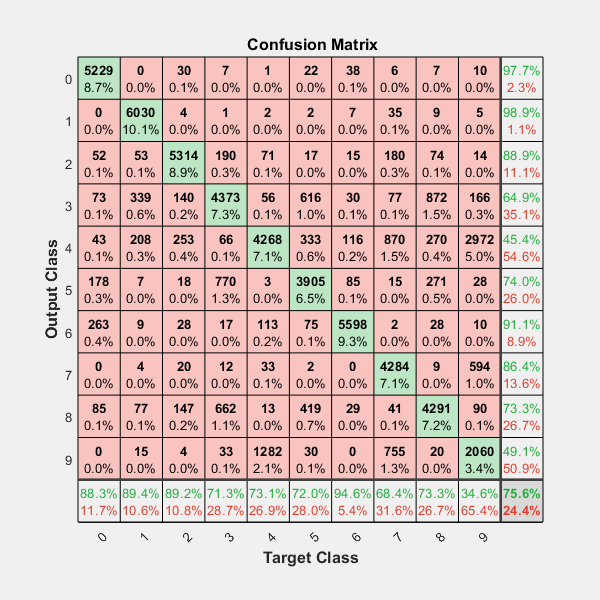
\includegraphics[scale=0.6]{figure_2.png}
\end{center}


\label{H_1D02A7CF}
\matlabheading{1.3 Plotting Learning Curves}

\begin{par}
\begin{flushleft}
By using psuedo-inverse algorithm we have found the weights at once, so there is no learning curve available to be displayed.
\end{flushleft}
\end{par}


\label{H_551432FF}
\matlabheading{1.4 Classification Performance}

\begin{par}
\begin{flushleft}
With the code snippet below, we first predict the labels of test dataset with the RBF network, then plot the confusion matrix to see how is the classification performance. 
\end{flushleft}
\end{par}

\begin{par}
\begin{flushleft}
As it is clear, performance on the whole test set of MNIST is about 76\% which is acceptable in comparison with the time that feed forward neural networks need to be trained and acheive a comparable performance. 
\end{flushleft}
\end{par}

\begin{matlabcode}
N_test = size(test_images_reshaped, 2);
hidden_test = zeros(N_test, K);

for i = 1:40
    hidden_test(:, i) = exp(vecnorm(test_images_reshaped'-centroids(i, :), 2, 2).^2/(-2*sigma*sigma));
end

predicted_test_labels_one_hot_encoded = hidden_test*weights;

[~, I] = max(predicted_test_labels_one_hot_encoded');

categorized_label_test = categorical(test_labels, 0:9, {'0' '1' '2' '3' '4' '5' '6' '7' '8' '9'});
categorized_label_test_predicted = categorical(I', 1:10, {'0' '1' '2' '3' '4' '5' '6' '7' '8' '9'});

plotconfusion(categorized_label_test, categorized_label_test_predicted);
\end{matlabcode}
\begin{center}
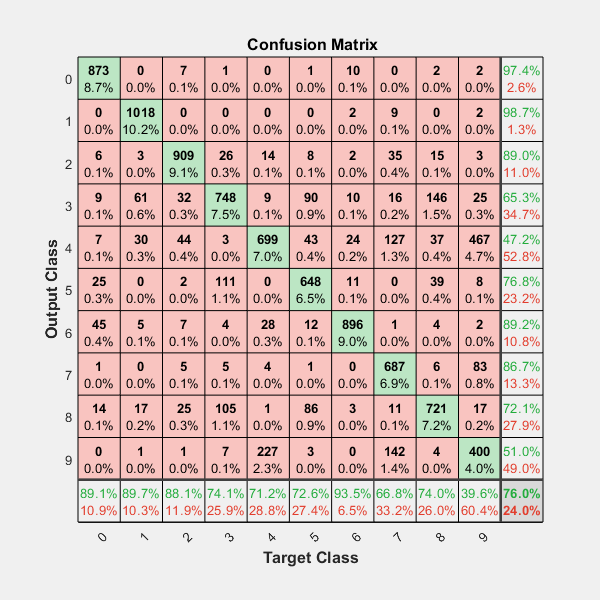
\includegraphics[scale=0.6]{figure_3.png}
\end{center}
\pagebreak

\label{T_6A4426AB}
\matlabtitle{Problem 2}
At first we rewrite the instantaneous error function as the equations below:

\begin{align*}
E(x^{(k)})&=\frac{1}{2}\{y^{(k)}-\sum_{i=1}^{m}w_i\exp[-\frac{||x^{(k)}-\mu_i||^2}{2\sigma_i^2}]\}^2\\ 
%&=\frac{1}{2}\{y^{(k)^2}+w_1^2\exp[-\frac{||x^{(k)}-\mu_1||^2}{\sigma_1^2}]+...+w_m^2\exp[-\frac{||x^{(k)}-\mu_m||^2}{\sigma_m^2}]\\
%&-2y^{(k)}w_1\exp[-\frac{||x^{(k)}-\mu_1||^2}{2\sigma_1^2}]-...-2y^{(k)}w_m\exp[-\frac{||x^{(k)}-\mu_m||^2}{2\sigma_m^2}]\\
%&+2w_1\exp[-\frac{||x^{(k)}-\mu_1||^2}{2\sigma_1^2}]w_2\exp[-\frac{||x^{(k)}-\mu_2||^2}{2\sigma_2^2}]+...+2w_1\exp[-\frac{||x^{(k)}-\mu_1||^2}{2\sigma_1^2}]w_m\exp[-\frac{||x^{(k)}-\mu_m||^2}{2\sigma_m^2}]\\
%&+...
%\}
\end{align*}

\matlabheading{2.1 Calculating $\mathbf{\partial E/\partial w_j}$}
We can immediately find this derivative by th compact form of the squared error equation.
\begin{align*}
\frac{\partial E}{\partial w_j}&=\frac{1}{2}(2)(y^{(k)}-\sum_{i=1}^{m}w_i\exp[-\frac{||x^{(k)}-\mu_i||^2}{2\sigma_i^2}])\exp[-\frac{||x^{(k)}-\mu_j||^2}{2\sigma_j^2}]\\
&=(y^{(k)}-f(x^{(k)}))\phi_j(x^{(k)})
\end{align*}

\matlabheading{2.2 Calculating $\mathbf{\partial E/\partial \mu_j}$}
\begin{align*}
\frac{\partial E}{\partial \mu_j}&=\frac{1}{2}(2)(y^{(k)}-\sum_{i=1}^{m}w_i\exp[-\frac{||x^{(k)}-\mu_i||^2}{2\sigma_i^2}])\frac{\partial}{\partial \mu_j}\{w_j\exp[-\frac{||x^{(k)}-\mu_j||^2}{2\sigma_j^2}]\}\\
&=(y^{(k)}-\sum_{i=1}^{m}w_i\exp[-\frac{||x^{(k)}-\mu_i||^2}{2\sigma_i^2}])w_j\exp[-\frac{||x^{(k)}-\mu_j||^2}{2\sigma_j^2}]\frac{\partial}{\partial \mu_j}\{-\frac{||x^{(k)}-\mu_j||^2}{2\sigma_j^2}\}\\
&=(y^{(k)}-\sum_{i=1}^{m}w_i\exp[-\frac{||x^{(k)}-\mu_i||^2}{2\sigma_i^2}])w_j\exp[-\frac{||x^{(k)}-\mu_j||^2}{2\sigma_j^2}](-\frac{2(x^{(k)}-\mu_j)}{2\sigma_j^2})\\
&=(y^{(k)}-f(x^{(k)}))\phi_j(x^{(k)})(-\frac{(x^{(k)}-\mu_j)}{\sigma_j^2})
\end{align*}

\matlabheading{2.3 Calculating $\mathbf{\partial E/\partial \sigma_j}$}
\begin{align*}
\frac{\partial E}{\partial \sigma_j}&=\frac{1}{2}(2)(y^{(k)}-\sum_{i=1}^{m}w_i\exp[-\frac{||x^{(k)}-\mu_i||^2}{2\sigma_i^2}])\frac{\partial}{\partial \sigma_j}\{w_j\exp[-\frac{||x^{(k)}-\mu_j||^2}{2\sigma_j^2}]\}\\
&=(y^{(k)}-\sum_{i=1}^{m}w_i\exp[-\frac{||x^{(k)}-\mu_i||^2}{2\sigma_i^2}])w_j\exp[-\frac{||x^{(k)}-\mu_j||^2}{2\sigma_j^2}]\frac{\partial}{\partial \sigma_j}\{-\frac{||x^{(k)}-\mu_j||^2}{2\sigma_j^2}\}\\
&=(y^{(k)}-\sum_{i=1}^{m}w_i\exp[-\frac{||x^{(k)}-\mu_i||^2}{2\sigma_i^2}])w_j\exp[-\frac{||x^{(k)}-\mu_j||^2}{2\sigma_j^2}](-(-2)\frac{||x^{(k)}-\mu_j||^2}{2\sigma_j^3})\\
&=(y^{(k)}-f(x^{(k)}))\phi_j(x^{(k)})(\frac{(x^{(k)}-\mu_j)}{\sigma_j^3})
\end{align*}

\pagebreak

\label{T_CB942182}
\matlabtitle{Appendix}

\label{H_EB7B647F}
\matlabheading{A.1 Saving Workspace Variables for Future Use }

\begin{matlabcode}
save('HW12_code_workspace.mat');
\end{matlabcode}


\label{H_23D8D399}
\matlabheading{A.2 Definition of Auxiliary Functions}

\begin{matlabcode}
function downloadMNIST(mnist_train_image, mnist_train_label, mnist_test_image, mnist_test_label)

if exist('train-images-idx3-ubyte','file') ~= 2
    disp('Downloading MNIST dataset...');
    websave([mnist_train_image,'.gz'],...
        ['http://yann.lecun.com/exdb/mnist/', ...
        mnist_train_image, '.gz']);
    websave([mnist_train_label,'.gz'],...
        ['http://yann.lecun.com/exdb/mnist/', ...
        mnist_train_label, '.gz']);
    websave([mnist_test_image,'.gz'],...    
        ['http://yann.lecun.com/exdb/mnist/', ...
        mnist_test_image, '.gz']);
    websave([mnist_test_label,'.gz'],...
        ['http://yann.lecun.com/exdb/mnist/', ...
        mnist_test_label, '.gz']);
    disp('MNIST dataset downloded.');
    
    disp('Unzipping started...');
    gunzip([mnist_train_image, '.gz'])
    gunzip([mnist_train_label, '.gz'])
    gunzip([mnist_test_image, '.gz'])
    gunzip([mnist_test_label, '.gz'])
    delete([mnist_train_image, '.gz'])
    delete([mnist_train_label, '.gz'])
    delete([mnist_test_image, '.gz'])
    delete([mnist_test_label, '.gz'])
    disp('Unzipping completed.');
else
    disp('MNIST dataset already downloaded.')
end

end

function [imgs, labels] = readMNIST(imgFile, labelFile, num_of_digits_to_read)

fileID = fopen(imgFile, 'r', 'b');
header = fread(fileID, 1, 'int32');

if header ~= 2051
    error('Invalid image file header');
end

count = fread(fileID, 1, 'int32');

if count < num_of_digits_to_read
    error('Trying to read too many digits');
end

rows_num = fread(fileID, 1, 'int32');
cols_num = fread(fileID, 1, 'int32');

imgs = zeros([rows_num cols_num num_of_digits_to_read]);

for i = 1:num_of_digits_to_read
    for row = 1:rows_num
        imgs(row, :, i) = fread(fileID, cols_num, 'uint8');
    end
end

fclose(fileID);

fileID = fopen(labelFile, 'r', 'b');
header = fread(fileID, 1, 'int32');

if header ~= 2049
    error('Invalid label file header');
end

count = fread(fileID, 1, 'int32');

if count < num_of_digits_to_read
    error('Trying to read too many digits');
end

labels = fread(fileID, num_of_digits_to_read, 'uint8');

fclose(fileID);

imgs = double(imgs)./255.0;

end

function iMontage(images)
montage(reshape(images, [28 28 size(images, 2)]), 'BackgroundColor', 'white', 'BorderSize', [2 2]);
end
\end{matlabcode}

\end{document}
